\chapter{Background and Related Work}
Before diving into the details of the pixel-based rendering approach with flow-based interpolation that is the focus of this thesis, it is important to outline the basic concepts and methods used in this approach (Section~\ref{sec:fundamentals}), as well as to understand the state-of-the-art of image-based rendering techniques (Section~\ref{sec:related_work}).

%\paragraph{Viewpoint, capture, camera} input viewpoint, output viewpoint
%captured viewpoint &=&  capture, synthesized viewpoint
%Capture/Viewpoint is the term used here to signify the location and image data of a 360\degree photograph taken at a certain position in the scene
%capture is more for when the images are actually recorded
%viewpoint is more for during processing
\section{Fundamentals}\label{sec:fundamentals}
The images used in this thesis, as well as many other approaches, are 360\degree images. Since 360\degree images differ significantly from ``regular'' images in how they are captured and visualized, it is important to understand how 360\degree cameras capture their surroundings, how the captured data can be mapped to a planar surface, and what the most common mappings for 360\degree images are (Section~\ref{subsec:fundamentals_360}). Also, the concept of optical flow is introduced, as it is a prerequisite for a number of image-based rendering techniques, including the flow-based interpolation used in this thesis (Section~\ref{subsec:optical_flow}).

\subsection{360\degree Images}\label{subsec:fundamentals_360}
Capturing an image with a 360\degree camera differs significantly from capturing an image with a regular camera. A regular camera captures incoming rays of light with a limited field of view. The sensors on the camera (or the film, for analog cameras), are arranged on a plane and register the wavelengths of incoming rays. This process represents a projection of the scene onto a plane. The measured light values can then be stored directly as a planar image (Figure~\ref{fig:cameras}a).


A 360\degree camera\footnote{The term ``omnidirectional camera'' is also used informally, however, this term is less exact, since an omnidirectional camera can also be a camera that captures a single hemisphere, instead of the full scene \cite{omnidir}.}, on the other hand, captures light rays with an field of view of 360$^{\circ}$. This means that the sensors are arranged in a way that captures light rays from the entire surroundings. For the sake of simplicity, this can be pictured as a number of sensors in the form of a sphere\footnotemark. The camera must then perform an additional conversion in order to transform the light values captured on a sphere to a planar image (Figure~\ref{fig:cameras}b). \cite{omnidir}

\footnotetext{The sensors cannot actually take the form of a perfect sphere, since the camera needs to have some form of casing. Instead, several lenses are usually used (``polydioptric cameras'' \cite{omnidir}), and the image stitched together in software.}

\begin{figure}[p]
\centering
    \begin{subfigure}[t]{0.9\textwidth}            
            \centering
            \includegraphics[width=\textwidth]{02/schematic01.png}
            \caption{Image capturing process with a regular camera: The sensors are arranged on a plane, so capturing the rays corresponds to a projection to a plane.}
    \end{subfigure}
    \begin{subfigure}[t]{0.9\textwidth}
            \centering
            \includegraphics[width=\textwidth]{02/schematic02.png}
            \caption{Image capturing process with a 360\degree camera: The sensors are arranged in an approximation of a sphere, which means an additional step is needed to convert the captured data to a planar representation.}
    \end{subfigure}
    \caption{Capturing an image with a regular camera compared to a 360\degree camera}\label{fig:cameras}
\end{figure}

The projection onto a flat surface is necessary, since image data is generally stored in 2D, and the majority of viewing devices are planar (e.g., computer or smartphone screens). The process of translating data from a 3D model to a 2D image and vice versa is well known in computer graphics and is called \emph{uv mapping} or \emph{texture mapping}.

Specifically, the process of \emph{uv mapping for spherical geometry} is needed to map the data from the sphere to a planar image. This process describes a bijective operation in which the points (x,y,z) on the sphere (described by \emph{unit directions} which are unit vectors) are associated with pixel positions in image coordinates (u,v). Figure~\ref{fig:uv_mapping} shows an example mapping between the unit sphere and a planar image. In this example, the poles of the sphere are mapped to the entire top and bottom pixel rows of the image, and the equator is mapped to the row of pixels in the vertical center of the image. This means that the areas near the poles are \emph{oversampled}, which indicates that the mapping function is not \emph{equal area} \cite[p.450]{hdrbook} i.e.\ it does not conserve how much area a pixel value occupies.

\begin{figure}[p]
		\centering
		\includegraphics[width=0.8\textwidth, keepaspectratio]{02/uv_mapping.png}
		\caption[UV mapping example]{Example of uv mapping for spherical geometry}
		\label{fig:uv_mapping}
\end{figure}

In the case of a 360\degree camera mapping the captured light rays to a planar image for storage, the image values are some type of color values. However, other kinds of information can also be uv-mapped to a shape, for example illumination data, depth values (``bump mapping''), and more.

%In the case of 360\degree images, the first step after capture is to convert the captured color values to a a planar image for storage and viewing.
%There are a number of common different mappings from which to choose from, depending on the application.
%\subsubsection{Common Mappings for 360\degree Images \cite[p. 535ff]{hdrbook}}\label{subsec:projections}
The most common mappings for 360\degree images are the \emph{cube map}, the \emph{ideal mirrored sphere}, the \emph{angular map},  and the \emph{equirectangular map} \cite[p. 535]{hdrbook}. The image data can be projected using any of these mappings with only minimal data loss from interpolation. These mappings are briefly presented in the following paragraphs.

\paragraph{Cube Map}
The cube map is a mapping that splits the image data into six separate square views, one in each direction (top, front, left, right, back, bottom). This is the equivalent of capturing the surroundings with six different cameras with a field of view of 90\degree each, and then stitching the resulting images into a shape that can be ``folded'' into a cube (see Figure~\ref{fig:cubemap-intro}), which also gives this mapping its name.

Due to the projection of a spherical surface to a plane, there is some distortion towards the edges of each face. However, this distortion is comparable to the distortion at the edges of a regular, planar image, which is a significant advantage compared to other mappings (see Figure\ref{fig:common_mappings}b,d,f,h\footnotemark). The disadvantage is that each face is projected separately, which leads to directional discontinuities at the many seams. This type of mapping is often used to simulate complex environments in 3D scenes (e.g., for game or animation graphics), as it is easy to use and reduces render time significantly compared to a 3D model of the same environment.

\footnotetext{Figure~\ref{fig:cubemap-distortion} does not perfectly represent the distortion in cube maps. It was chosen as a baseline because cube maps have relatively little distortion compared to other mappings and it visualizes which parts of the image are mapped where and how they are distorted in other mappings.}
\cite[p. 540]{hdrbook}

\paragraph{Ideal Mirrored Sphere}
The ideal mirrored sphere is a mapping to a circle within a square (see Figure~\ref{fig:sphere-intro}). It represents how the surroundings would be reflected if one placed a small sphere with a perfectly reflective surface (``mirrored'' sphere) into a scene and then photographed it using an orthographic camera. This mapping, like all the mappings presented here, shows the complete surroundings, albeit considerably distorted toward the edges. Figure~\ref{fig:sphere-distortion} shows where each direction is mapped and the extent of the distortion. It is clear that the farther away from the ``front'' area, the more distorted the mirrored sphere mapping is. The ideal mirrored sphere mapping can be used for calculating average illumination color for high dynamic range calculations; however, the type of distortion at the edges can cause problems with sampling, which is why the angular map mapping tends to be preferred.
\cite[p. 535]{hdrbook}

\paragraph{Angular Map}
At first sight, the angular map seems very similar to the ideal mirrored sphere. It also maps to a circle within a square, however it samples the input in such a way that the back of the image is allotted more space and is less distorted than the mirrored sphere (see Figure~\ref{fig:angular-intro} and Figure~\ref{fig:angular-distortion}).
\cite[p. 537]{hdrbook}

\paragraph{Equirectangular Map}
The equirectangular, or latitude-longitude (``latlong'') mapping is a common type of mapping in cartography. The data is mapped to a rectangular image space, in which the width is twice the height. The azimuth (around the circumference) of the unit directions is mapped to the map's horizontal coordinate and the elevation to the vertical coordinate (see Figure~\ref{fig:latlong-intro}). The main problem of this representation is well known in cartography: The distortion increases significantly towards the poles, as can be seen in Figure~\ref{fig:latlong-distortion}. Otherwise, this mapping is convenient as it has very few seams and all pixels are valid (i.e.\ there are no ``black'' areas). It is used as a storage format for 360\degree images.
\cite[p. 538]{hdrbook}

\paragraph*{}
While all of these projections are static, showing the entirety of the 360\degree image at once, it is also possible to view 360\degree images interactively. In this case the field of view tends to be limited, so only a certain part of the image needs to be projected: the part of the image the viewer is ``facing'' virtually. Once the viewing direction has been determined, the projection can be calculated such that the center of the image has minimal distortion. Theoretically, any of the above projections could be used for this. 

\begin{figure}
\centering
    \hfill
    \begin{subfigure}[t]{0.5\textwidth}            
            \centering
            \includegraphics[width=0.7\textwidth, keepaspectratio]{02/mapping_cube_photo.jpg}
            \caption{Cube map example}\label{fig:cubemap-intro}
    \end{subfigure}%
    \hfill
    \begin{subfigure}[t]{0.5\textwidth}
            \centering
            \includegraphics[width=0.7\textwidth, keepaspectratio]{02/mapping_cube.jpg}
            \caption{Cube map distortion visualization}\label{fig:cubemap-distortion}
  
    \end{subfigure}
    \hfill
    \par\bigskip % maximise vertical space here instead

    \hfill
    \begin{subfigure}[t]{0.5\textwidth}
            \centering
            \includegraphics[width=0.5\textwidth, keepaspectratio]{02/mapping_sphere_photo.jpg}
            \caption{Mirrored sphere mapping example}
            \label{fig:sphere-intro}
    \end{subfigure}%
    \hfill
    \begin{subfigure}[t]{0.5\textwidth}
            \centering
            \includegraphics[width=0.5\textwidth, keepaspectratio]{02/mapping_sphere.jpg}
            \caption{Mirrored sphere distortion visualization}
            \label{fig:sphere-distortion}
    \end{subfigure}
    \hfill
    \par\bigskip % maximise vertical space here instead

    \hfill
    \begin{subfigure}[t]{0.5\textwidth}            
            \centering
            \includegraphics[width=0.5\textwidth, keepaspectratio]{02/mapping_angular_photo.jpg}
            \caption{Angular mapping example}
            \label{fig:angular-intro}
    \end{subfigure}%
    \hfill
    \begin{subfigure}[t]{0.5\textwidth}
            \centering
            \includegraphics[width=0.5\textwidth, keepaspectratio]{02/mapping_angular.jpg}
            \caption{Angular mapping distortion visualization}
            \label{fig:angular-distortion}
    \end{subfigure}
    \hfill
    \par\bigskip % maximise vertical space here instead

    \hfill
    \begin{subfigure}[t]{0.5\textwidth} 
            \centering
            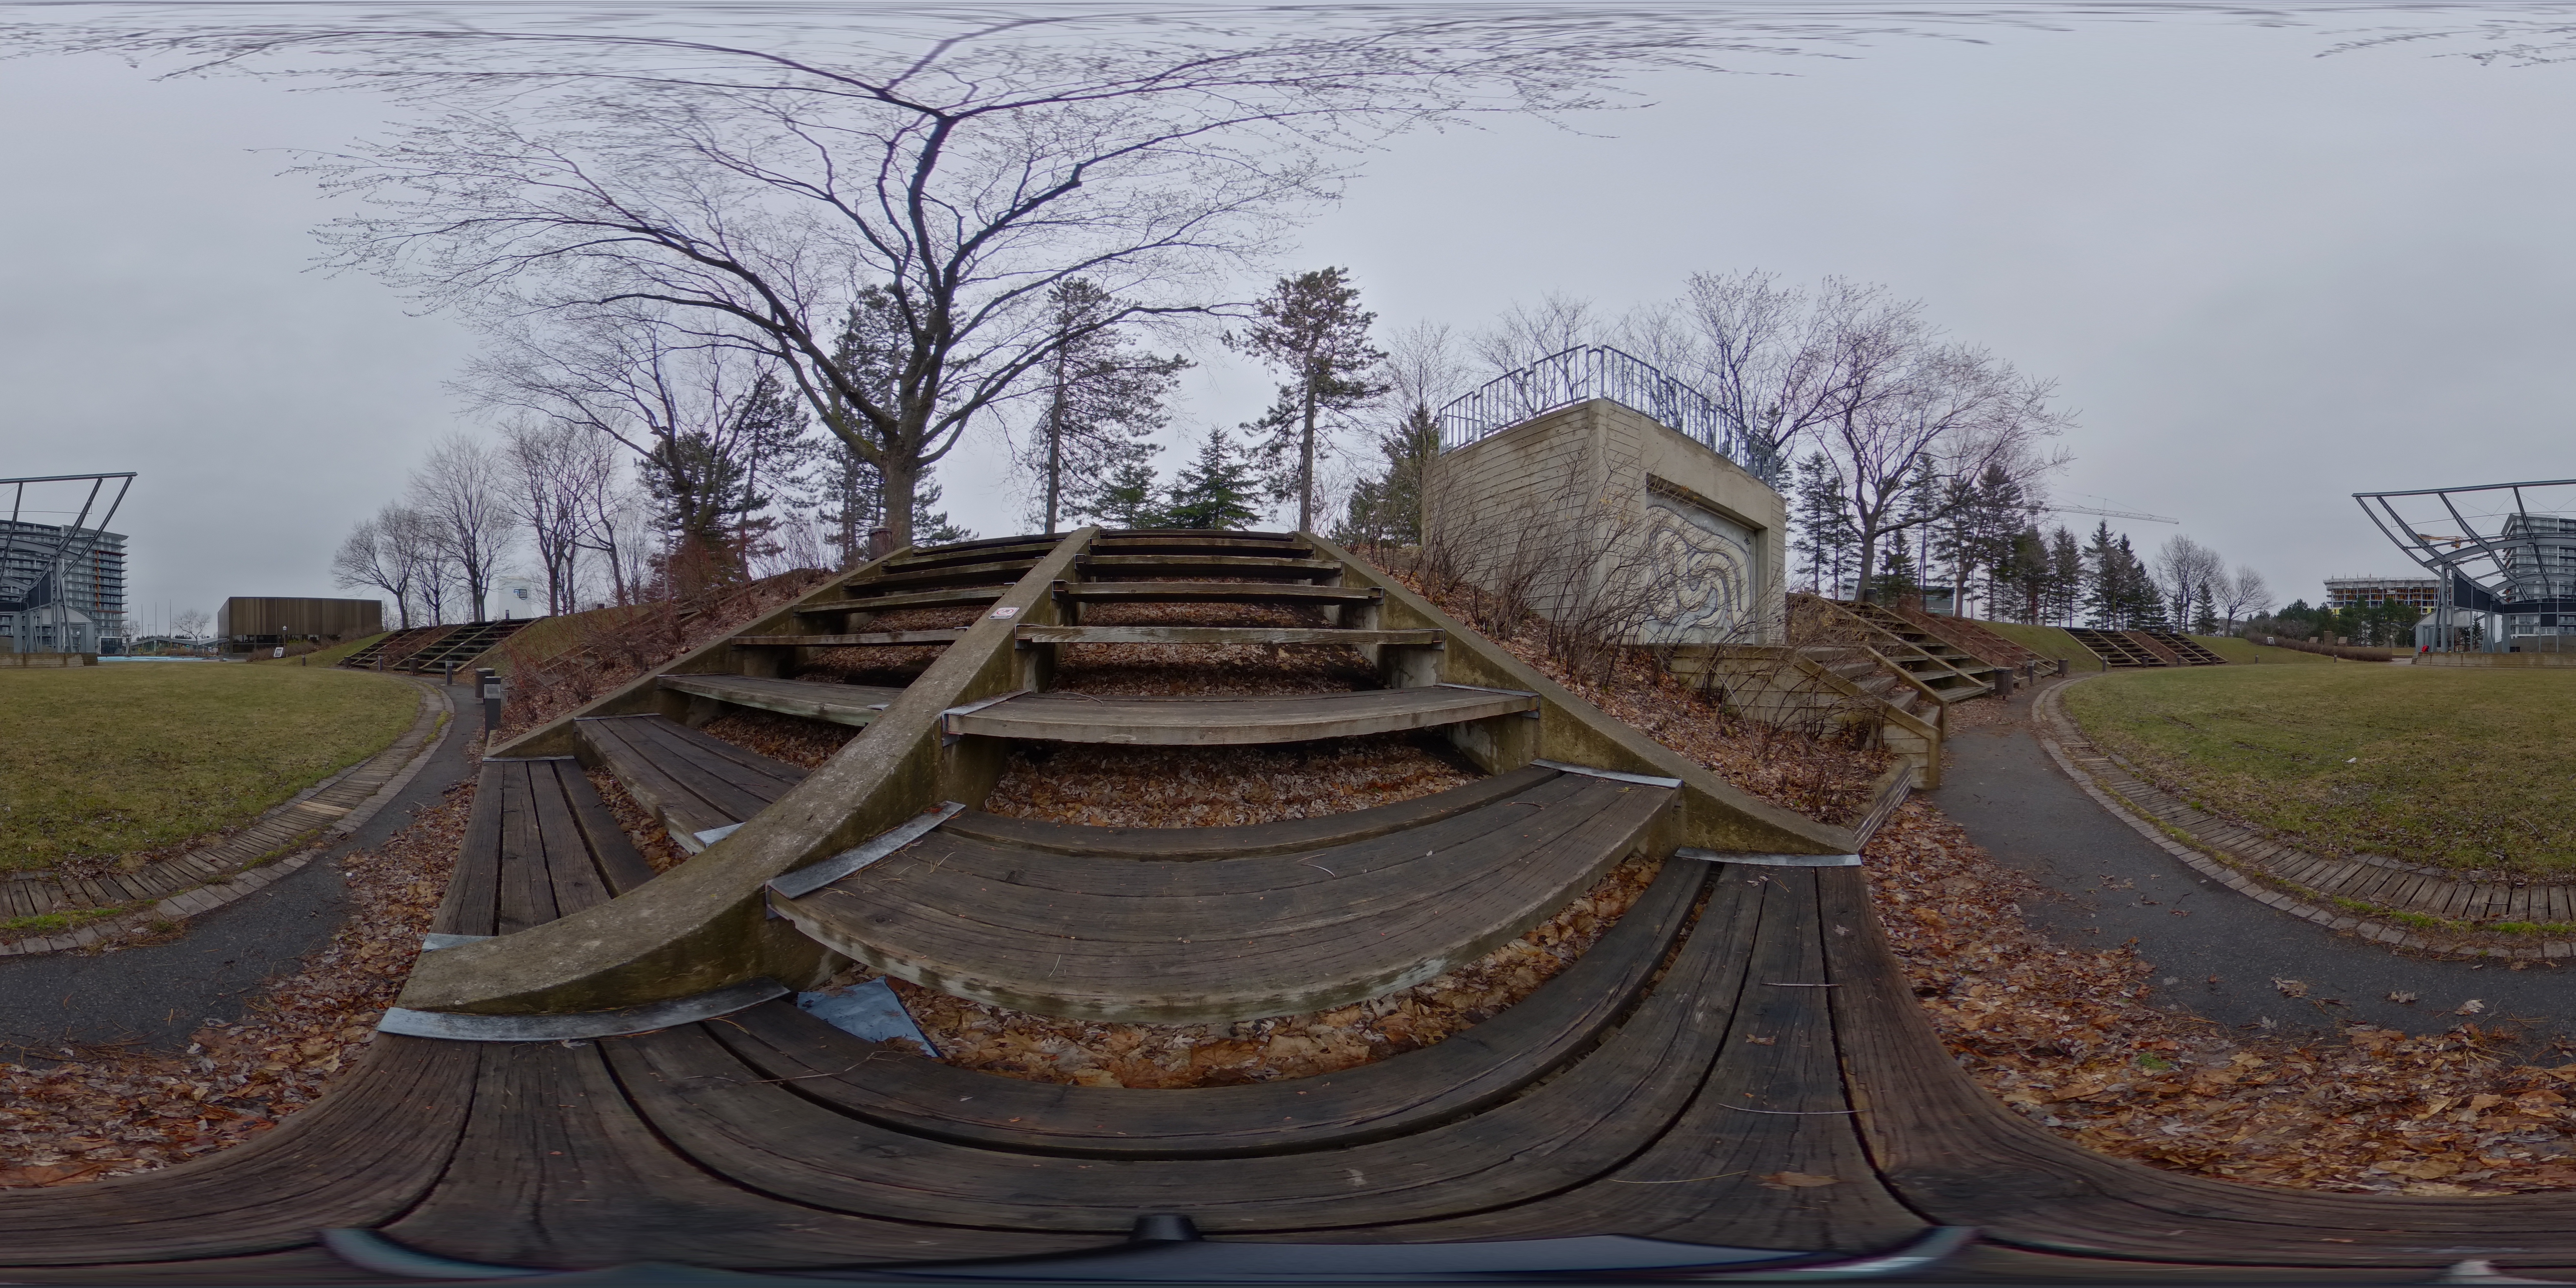
\includegraphics[width=0.9\textwidth, keepaspectratio]{02/mapping_latlong_photo.jpg}
            \caption{Equirectangular (latlong) mapping example}
            \label{fig:latlong-intro}
    \end{subfigure}%
    \hfill
    \begin{subfigure}[t]{0.5\textwidth}
            \centering
            \includegraphics[width=0.9\textwidth, keepaspectratio]{02/mapping_latlong.jpg}
            \caption{Equirectangular distortion visualization}
            \label{fig:latlong-distortion}
    \end{subfigure}
    \hfill
    \caption{Common mappings for 360\degree images}\label{fig:common_mappings}
  \end{figure}
  
\subsection{Optical Flow} \label{subsec:optical_flow}
Optical flow describes the displacement of specific points between two images. It is generally used on consecutive frames of video sequences, for example for semantic segmentation, structure-from-motion, data compression or other applications where information about movement between images is required. To illustrate, Figure~\ref{fig:of_example_bike} shows two consecutive frames of a video sequence. On a high level, an optical flow algorithm should recognize that the pixels representing the bicyclist are moving towards the bottom left of the image, and the pixels representing the background are moving to the right (because the camera is panning slightly to the left).

There are two types of optical flow: sparse optical flow and dense optical flow. Sparse optical flow algorithms calculate the motion of several select points that can be either chosen manually, or by some kind of automatic selection (e.g., based on features). This type of optical flow can be used to track only specific objects in a scene (e.g., the direction and relative velocity of a certain car in traffic).

Dense optical flow algorithms compute the motion of \emph{each pixel} between two images, instead of single points. This can be used for more general object tracking (e.g., direction and relative velocity of complete surroundings in traffic), to estimate 3D geometry (in structure-from-motion algorithms), or to identify static sections of the image for video compression \cite{of-survey}. Dense optical flow can also be used for image synthesis, such as in Richardt et al's Megastereo \cite{megastereo} described in Section~\ref{subsec:megastereo}, which is also the basis of the flow-based interpolation presented in this thesis.

There are a number of optical flow algorithms, ranging from methods using parametrization, or regularization \cite{of-survey} to methods relying on Deep Learning \cite{of-deep}. Although these algorithms differ greatly in approach, they share the type of result, which is a vector field. For dense optical flow, this vector field contains a vector for each pixel, describing the displacement of this pixel between the input images. Sparse optical flow only contains a vector for each pre-chosen point, not for every pixel.

Figure~\ref{fig:of_vis} shows two different visualizations of the vector field calculated by the dense optical flow algorithm by Farneb\"ack \cite{farneback} between the frames in Figure~\ref{fig:of_example_bike}. Figure~\ref{fig:of_vis}a is a color-based visualization: the hue encodes the vector direction and the saturation encodes the vector length for each pixel. Using this visualization, it is possible to roughly distinguish two separately moving areas of the image, which could be used for semantic segmentation. Figure~\ref{fig:of_vis}b shows the pixel displacements with vectors: The vector orientations and lengths are represented by arrows.

These visualizations can help show if and how well an optical flow algorithm is working. Although there are a large number of different algorithms, most of them still do not effectively deal with common issues such as occlusions, too-large displacements and intensity changes \cite{of-survey}. Occlusions are problematic, since the displacements between two images may reveal or cover image areas that, as a result, have no correspondence in the previous image. This problem is exacerbated when displacements are very large (e.g., due to fast-moving objects). Large displacements are also problematic by their very nature, as most algorithms are not designed to handle them. How these limitations affect the use of optical flow for image synthesis will be discussed in Chapters~\ref{chap:implementation} and \ref{chap:evaluation}.

\begin{figure}
\centering
    \hfill
    \begin{subfigure}[b]{0.45\textwidth}            
            \centering
            \includegraphics[width=\textwidth, keepaspectratio]{02/of_example1.jpg}
            \caption{Frame 1}
    \end{subfigure}%
    \hfill
    \begin{subfigure}[b]{0.45\textwidth}
            \centering
            \includegraphics[width=\textwidth, keepaspectratio]{02/of_example2.jpg}
            \caption{Frame 2}
    \end{subfigure}
    \hfill
    \caption[Optical flow example]{Example frames that optical flow is calculated on}\label{fig:of_example_bike}
    \par\bigskip

    \hfill
    \begin{subfigure}[b]{0.45\textwidth}            
            \centering
            \includegraphics[width=\textwidth, keepaspectratio]{02/of_vis1.jpg}
            \caption{Visualization of optical flow with color: the hue encodes the vector direction, the saturation encodes the vector length for each pixel.}
    \end{subfigure}%
    \hfill
    \begin{subfigure}[b]{0.45\textwidth}
            \centering
            \includegraphics[width=\textwidth, keepaspectratio]{02/of_vis2.jpg}
            \caption{Visualization of optical flow with arrows: The vectors are represented by arrows (only a limited number of vectors are shown)}
    \end{subfigure}
    \hfill
    \caption[Optical flow visualizations]{Optical flow visualizations}\label{fig:of_vis}
\end{figure}

\section{Related Work}\label{sec:related_work}
Image-based rendering (IBR) and viewpoint interpolation\footnotemark\ started attracting interest with the advent of virtual walkthroughs, for example for Apple's QuickTime\textsuperscript{\textregistered} VR, in order to save render time by generating views from images instead of using complex 3D scenes including textures, lights and complex geometric models \cite{quicktime}.
Chen and Zhang, in their survey on image-based rendering \cite{survey2004}, use the terms \emph{source description} and \emph{appearance description} to compare these basic rendering techniques: ``Traditional'' rendering techniques use \emph{source description}, i.e.\ the scene is described by the objects within it, their positions and properties. On the other hand, IBR techniques try to achieve the same goal through \emph{appearance description}:
Instead of trying to describe the scene through the objects it contains, image-based rendering techniques try to model the \emph{light rays} that reach the viewer.
The reason why this is feasible is that human vision itself has little to do with 3D geometry; it is the processing of a dense set of light rays by the brain which are ``captured'' by the eye. This process can also be performed by a capture device like a camera. As a result, it is not necessary to meticulously model the source, it is sufficient to model the ``appearance'' (i.e., the light rays) of a scene.
%Vision itself has little to do with 3D geometry; it is the processing of a dense set of light rays by the brain which are ``captured'' by the eye. This process can also be performed by a capture device like a camera. So, instead of trying to describe the scene through the objects it contains, IBR rendering techniques try to model the \emph{light rays} that reach the viewer. 

\footnotetext{As there seems to be no explicit difference between the terms ``image-based rendering'', ``viewpoint interpolation'' and ``viewpoint synthesis'' in the literature, they will be used interchangeably in this thesis, although ``interpolation'' is favored for simpler blending techniques, and ``synthesis'' is used to describe more complex algorithms.}

While the differentiation between source description and appearance description is helpful in understanding the basic differences between image-based and traditional rendering, many image-based rendering methods also utilize some form of source description, predominantly in the form of 3D geometry. In a different survey on image-based rendering techniques, Kang and Shum \cite{survey2000} classify IBR rendering techniques on a continuum, which ranges from techniques using no geometry, to techniques using implicit geometry (or more generally, feature correspondences), to techniques using explicit geometry. %(see Figure~\ref{fig:survey_categorization}).

%\begin{figure}
%		\centering
%		\includegraphics[width=\textwidth]{02/shum_kang_survey.png}
%    \caption[Categorization of IBR techniques from \cite{survey2000}]{Categorization of IBR techniques with representative members, taken from Kang and Shums ``A Review of Image-based Rendering Techniques''\cite{survey2000}}
%		\label{fig:survey_categorization}
%\end{figure}

The algorithm presented in this thesis is a combination of two different approaches: the first step uses no geometry whatsoever, and the second step uses feature correspondences to correct some of the problems that arise in the first step. This differentiation guides the related work presented here: The first section presents synthesis approaches using no geometry, and the second section presents approaches using implicit geometry or feature correspondences.

%\begin{itemize}
%  \item type of warping: uv mapping, warping based on triangulation and homography
%  \item image representation: cube, planar, sphere
%  \item constraints? color / angle / \ldots
%  \item geometry? sparse, dense, none
%  \item correspondences needed? sparse, dense, none
%  \item type of input: planar, 360, 180 pano
%  \item type of output: planar, 360, 180 pano
%\end{itemize}

\subsection{Image Synthesis without Image Correspondences}
A theoretical model for image synthesis with no geometry or other image features (i.e., ``pure'' appearance description) was developed by Adelson et al.\ \cite{Adelson91}: the \emph{plenoptic function} (Equation~\ref{eq:plenoptic}). The plenoptic function is a 7D function that describes the observable light at every point in space $V_x$, $V_y$, $V_z$, from every direction $\theta$, $\varphi$, at every wavelength $\lambda$, at every possible point in time $t$.

\begin{equation}
  \label{eq:plenoptic}
  P = P(\theta, \varphi, \lambda, t, V_x, V_y, V_z)
\end{equation}

In practice, it is infeasible, if not impossible, to cover all dimensions of this function, as this would require a capture device at every location, at every point in time, capturing light rays coming from every direction. However, by making different assumptions, IBR techniques try to reconstruct simplified versions of the plenoptic function. Common assumptions are the reduction of wavelengths to RGB, the removal of the temporal dimension, and the assumption that the light is constant along a ray in empty space (i.e., light does not change its wavelength over distance) \cite{survey2004}.
The methods for resampling the plenoptic function, or a lower-dimensional version are diverse, from Light Field Rendering \cite{lightfield}, which uses a capturing rig to uniformly sample the surroundings with a very high sample rate, and is able to construct views in real time, to more recent approaches that use neural networks to enhance the captured samples \cite{cnn}, or even predict light fields, or ``radiance fields'', themselves \cite{nerf}. The following section presents approaches that concern themselves specifically with 360\degree images, as this is most relevant for this thesis.

\subsubsection{``A Simple Method for Light Field Resampling'' \cite{simple_poster}}
Kawai \cite{simple_poster} approaches the problem of synthesizing new images with two degrees of freedom without using 3D geometry. Their basic setup is to capture four 360\degree images at each corner of a rectangular area and use resampling to synthesize a new image anywhere within this area.

The resampling is done by inserting a virtual sphere centered at the synthesized viewpoint representing a projection screen on which to project rays from the captured viewpoints. The locations of the captured viewpoints are known, so the outbound rays of these viewpoints can be calculated by using the image-to-world coordinate conversion from the equirectangular representation. The intersections of these captured rays with the virtual sphere are calculated and the corresponding pixel values are used. The projection screen where no rays have intersected are approximated by repeating the reprojection at different resolutions.

In cases where several rays share an intersection, Kawai proposes several methods. The first is to take an average of the rays. As an alternative, they suggest employing a rating based on the inner product of the ray direction and the viewing direction and using the ray with the smallest score. A final option is to prioritize one specific captured viewpoint over the others to completely avoid ghosting artefacts.

To evaluate their method they capture four viewpoints in a scene (the distances between the viewpoints are not mentioned) and calculate an image along a diagonal. They then compare the results of the different ray combination methods by describing visual artefacts.

\subsubsection{``On the Use of Ray-tracing for Viewpoint Interpolation in Panoramic Imagery'' \cite{raytracing}}
%correspondences needed: none, geometry: none/dense, constraints: color-constraint, image rep: cube, type of warping: pixel blending
Shi et al.\ \cite{raytracing} examine how ray tracing can be used to calculate arbitrary new viewpoints based on knowledge of relative positions between the viewpoints which are stored as cube maps. For every pixel in the target image, a ray is cast into the scene. Since the geometry of the scene is unknown, an alternative method is used to find the correct value of that point. They do this by introducing a color consistency constraint, which compares the pixel values of the rays cast from all the reference images. The assumption is that if the colors of different rays are the same, the rays must be intersecting the same point.

In order to calculate an intersection with the scene, they propose two different methods: a brute-force depth search using no scene geometry which searches along all of the captured rays until the pixel values are similar enough to fulfill their color constraint requirements, or a guided depth search using sparse 3D reconstruction.

To evaluate their method, they use a set of five captured input images with a maximum distance of one meter, from which they remove one to use as ground truth. They evaluate the algorithm by comparing the brute-force to the guided depth search based on the artefacts in the results and the computation time.

\subsubsection{``Unconstrained Segue Navigation for an Immersive Virtual Reality Experience'' \cite{segue}}
Herath et al.\ \cite{segue} propose a system that enables casual users to capture their surroundings in a grid with a smartphone, and then navigate that environment with two degrees of freedom. In order to interpolate between two captured 360\degree images (1-DoF), they differentiate between faces that are parallel to the axis of movement and faces that are perpendicular to the axis of movement. For faces that are parallel, they stitch the faces of two adjacent viewpoints together and interpolate by using a sliding window. For faces that are perpendicular, they calculate a homography between the faces of two adjacent viewpoints and morph the image accordingly. To interpolate any image within a rectangular area bounded by four captured viewpoints (2-DoF), they recursively interpolate intermediary viewpoints until they reach the desired position.

As the focus of this work is on the whole process of capture, navigation, and viewing, the interpolation step is not explicitly evaluated.

\subsection{Image Synthesis using Image Correspondences}
Leveraging image correspondences for synthesis has been a popular method almost since the beginning of viewpoint synthesis. Chen and Williams \cite{apple} were one of the first to use ``the morphing method'' that simultaneously blends the shape and texture of two images using image correspondences. A comparable method, based on optical flow, is used by Richardt et al.\ \cite{megastereo} for planar images.

Adaping planar algorithms (e.g., optical flow, structure-from-motion) for 360\degree images is a common challenge in 360\degree image synthesis. Kolhatkar et al.\ \cite{360flowblending} and Huang et al.\ \cite{6dof} solve this problem by extending the faces of the cube maps to account for pixels moving across borders. \cite{360flowblending} then use optical flow for interpolation between two images; whereas \cite{6dof} estimates the scene geometry with a structure-from-motion algorithm to extend monoscopic 360\degree videos to stereo. Zhao et al.\ \cite{cube2video} propose a method for adapting sparse correspondence matching for the spherical domain, circumventing the need to use an extended cube map.

Morphing the images to create a new viewpoint can be done with pixel-based blending \cite{megastereo}, \cite{360flowblending} or by triangulating the image and calculating homographies between the triangles \cite{6dof}, \cite{cube2video}.

%, and \cite{360flowblending} for 360\degree images, whose approaches are very similar to the flow-based blending step presented in this thesis.

%- triangulation based on correspondences + homographical morphing

The flow-based blending approach in this thesis builds on the approaches of \cite{megastereo} and \cite{360flowblending}, which are presented in more detail in the following sections.

\subsubsection{``Megastereo: Constructing High-Resolution Stereo Panoramas'' \cite{megastereo} \label{subsec:megastereo}}
%correspondences needed: dense, geometry: none, constraints: angle?, image rep: planar, type of warping: none, because planar
Richardt et al.\ \cite{megastereo} present an approach which combines planar images captured casually on a radius to create a panoramic image that is viewable in stereo in high resolution. In place of scene geometry, they use a cylindrical imaging surface that is concentric to the capture center. For each eye at a given viewing orientation, they project a ray into the scene (Figure~\ref{fig:megastereo}a) and calculate the deviation angle $\alpha$ between the desired ray and the nearest captured rays (Figure~\ref{fig:megastereo}b). 

\begin{figure}[]
\centering
\includegraphics[width=1\textwidth, keepaspectratio]{02/megastereo-figure.png}
\caption[Flow-based blending in Megastereo \cite{megastereo}]{(a) Illustration of rays required for creating a stereoscopic panorama and (b) deviation angles $\alpha$. (c) Duplication and truncation artefacts caused by the aliasing. (d) Flow-based upsampling to synthesize required rays. \emph{Adapted from \cite{megastereo}}}
\label{fig:megastereo}
\end{figure}

Because linearly blending the rays of the two closest captures would lead to artefacts due to the difference between the real geometry and the cylindrical surface (Figure~\ref{fig:megastereo}c), and using a nearest-neighbor technique would result in discontinuities, they propose a ``flow-based blending'' technique: For each ray of the final image that is not a captured ray (deviation angle 0), a new ray is synthesized using optical flow. The vertical image strip captured by the synthesized ray is interpolated by taking the two closest viewpoints $I_K$ and $I_L$ and interpolating $\widetilde{I_M}$ (Figure~\ref{fig:megastereo}d) using the optical flow vectors $F_{k\rightarrow l}$ and $F_{l\rightarrow k}$.  The corresponding strip is then taken from this new viewpoint which contains the matching ray.

%use a combination of image stitching and their own optical flow-based blending algorithm in order to account for . The goal is to synthesize stereoscopic viewpoints (an image for the left and right eye, each) from the set of captured monoscopic images. For the image strips for which a matching ray was not captured, they introduce a blending algorithm based on optical flow.

%After transforming the images so that they all have scene-independent orientation and minimal distortion, strips of the captured images are extracted for each ``eye'' based on the best matching image ray (Figure~\ref{fig:megastereo-figure}a and b). In cases where there is no perfect ray correspondence, the ray with the smallest deviation angle can be chosen, however, this can lead to artefacts as illustrated in Figure~\ref{fig:megastereo-figure}c. In order to mitigate these artefacts, Richardt et al.\ introduce a blending algorithm based on optical flow: 

%For Megastereo, there is no need to blend the complete images, instead, they restrict their calculations to the strips/pixels they need. For simplicity's sake, the process is described for a full image:
The interpolated image $\widetilde{I_M}$ at point $\eta$ between the images $I_K$ and $I_L$ is calculated by shifting $I_K$ by $\eta \cdot F_{k\rightarrow l}$ and by shifting $I_L$ by $(1 - \eta) \cdot F_{l\rightarrow k}$. The two shifted images are then blended linearly, using $\eta$ as the weight. Instead of calculating the entire image for each ray, only the necessary image areas are extracted and the interpolation is calculated pixel-wise.

To evaluate their method, they leverage datasets used by other approaches, as well as capturing their own images. They visually compare the results, noting improvements based on visible artefacts.

%According to the authors, their approach ``can handle angular resolutions from 1\degree to 4\degree, but even 8\degree produces agreeable results''. Although the approach is designed for planar images, the idea of leveraging deviation angles for  flow-blending approach is used 


\subsubsection{``Real-Time Virtual Viewpoint Generation on the GPU for Scene Navigation'' \cite{360flowblending}}
Kolhatkar and Lagani\`ere \cite{360flowblending} propose a method for smoothly interpolating between pairs of 360\degree images.
Their approach is similar to the approach in Megastereo, where optical flow between the images is used to incrementally morph the two images. In order to adapt the optical flow calculation for 360\degree images, they extend the cube map representation to account for points moving across edges, which is the method that is used in this thesis, as well. To reduce artefacts in the obtained optical flow, they perform a matching and smoothing step. They then implement their algorithm on the GPU, which allows them to interpolate between images in real-time. 

They evaluate their method by capturing scenes at ``reasonable'' distances and removing every other image in order to obtain ground truth data. The computation time of the optical flow calculation of the extended cubes is measured, as well as the actual interpolation time. Furthermore, they compare the interpolated results with ground truth images, both visually and by using a per-pixel metric.

\subsection{Discussion}
The overview of the presented approaches (Table~\ref{tab:comparison}) show that of the presented approaches, most of the approaches using feature correspondences only allow for synthesis with 1-DoF, whereas the approaches using no correspondences allow for synthesis with 2-DoF. There is no approach that attempts image synthesis in 2-DoF using optical flow.

As for the evaluation, none of the approaches test their methods on a defined parameter space. The only approaches that declare which parameters were used for the presented examples are \cite{raytracing} and \cite{cube2video} (marked in parentheses). Almost all approaches examine their results visually, remarking on artefacts, but only two use dedicated mathematical error metrics. All of the approaches evaluate the computational cost, whether they have a real-time requirement or not. Finally, only \cite{megastereo}, \cite{6dof} and \cite{cube2video} compare their methods to other approaches. In general, the evaluations presented in the approaches are mostly based on a very small sample set, and are not methodical, or necessarily well-defined.

\begin{table}[]
  \resizebox{\columnwidth}{!}{
\begin{tabular}{|c|c|c|c|c|c|c|c|c|}
\hline
\multirow{2}{*}{\textbf{}} & \multicolumn{3}{c|}{\textbf{method}} & \multicolumn{5}{c|}{\textbf{evaluation}} \\ \cline{2-9} 
 & \textbf{\begin{tabular}[c]{@{}c@{}}input\\ type\end{tabular}} & \textbf{DoF} & \textbf{\begin{tabular}[c]{@{}c@{}}extracted\\ features\end{tabular}} & \textbf{\begin{tabular}[c]{@{}c@{}}defined\\ parameter\\ space?\end{tabular}} & \textbf{\begin{tabular}[c]{@{}c@{}}visual\\ eval.\end{tabular}} & \textbf{\begin{tabular}[c]{@{}c@{}}error\\ metrics\end{tabular}} & \textbf{\begin{tabular}[c]{@{}c@{}}compu-\\ tational\\ cost\end{tabular}} & \textbf{\begin{tabular}[c]{@{}c@{}}comparison\\ to other\\ approaches\end{tabular}} \\ \hline
\cite{simple_poster} & \begin{tabular}[c]{@{}c@{}}360\degree\\ images\end{tabular} & 2 & none & \cross & \checkm & \cross & \checkm & \cross \\ \hline
\cite{raytracing} & \begin{tabular}[c]{@{}c@{}}360\degree\\ images\end{tabular} & 2 & \begin{tabular}[c]{@{}c@{}}none/\\ dense geo\end{tabular} & (\cross) & \checkm & \cross & \checkm & \cross \\ \hline
\cite{segue} & \begin{tabular}[c]{@{}c@{}}360\degree\\ images\end{tabular} & 2 & none & \cross & \cross & \cross & \checkm & \cross \\ \hline
\cite{megastereo} & \begin{tabular}[c]{@{}c@{}}planar\\ images\end{tabular} & 1 & \begin{tabular}[c]{@{}c@{}}dense\\ flow\end{tabular} & \cross & \checkm & \cross & \checkm & \checkm \\ \hline
\cite{360flowblending} & \begin{tabular}[c]{@{}c@{}}360\degree\\ images\end{tabular} & 1 & \begin{tabular}[c]{@{}c@{}}dense\\ flow\end{tabular} & \cross & \checkm & \checkm & \checkm & \cross \\ \hline
\cite{6dof} & \begin{tabular}[c]{@{}c@{}}360\degree\\ video\end{tabular} & 3* & \begin{tabular}[c]{@{}c@{}}dense\\ geo\end{tabular} & \cross & \checkm & \cross & \checkm & \checkm \\ \hline
\cite{cube2video} & \begin{tabular}[c]{@{}c@{}}360\degree\\ video\end{tabular} & 1 & \begin{tabular}[c]{@{}c@{}}sparse\\ feature\end{tabular} & (\cross) & \checkm & \checkm & \checkm & \checkm \\ \hline
\multicolumn{9}{r}{*on a constrained path}
\end{tabular}
}
\caption{Comparing the methods and evaluations of different approaches}\label{tab:comparison}
\end{table}
